\begin{frame}
  \frametitle{\textbf{Strangeness Enhancement in HI Collisions}}

  \begin{columns}
    

    \column{0.5\textwidth}
    \centering
    \begin{itemize}
    \item QGP state $\to$ increased production of $s$ and $\bar{s}$ quarks
    \item Expect an yield-increase in strange particles
      \begin{itemize}
      \item $\Lambda(uds)$, $\bar{\Lambda}(\bar{u}\bar{d}\bar{s})$
      \item $\Xi(dss)$, $\bar{\Xi}(\bar{d}\bar{s}\bar{s})$
      \item $\Omega(sss)$, $\bar{\Omega}(\bar{s}\bar{s}\bar{s})$
      \end{itemize}
    \item Enhancement increases with strangeness and multiplicity $\to$ \textbf{consistent with QGP formation}
    \end{itemize}

    \column{0.5\textwidth}
    \centering
    \begin{tikzpicture}
      \node{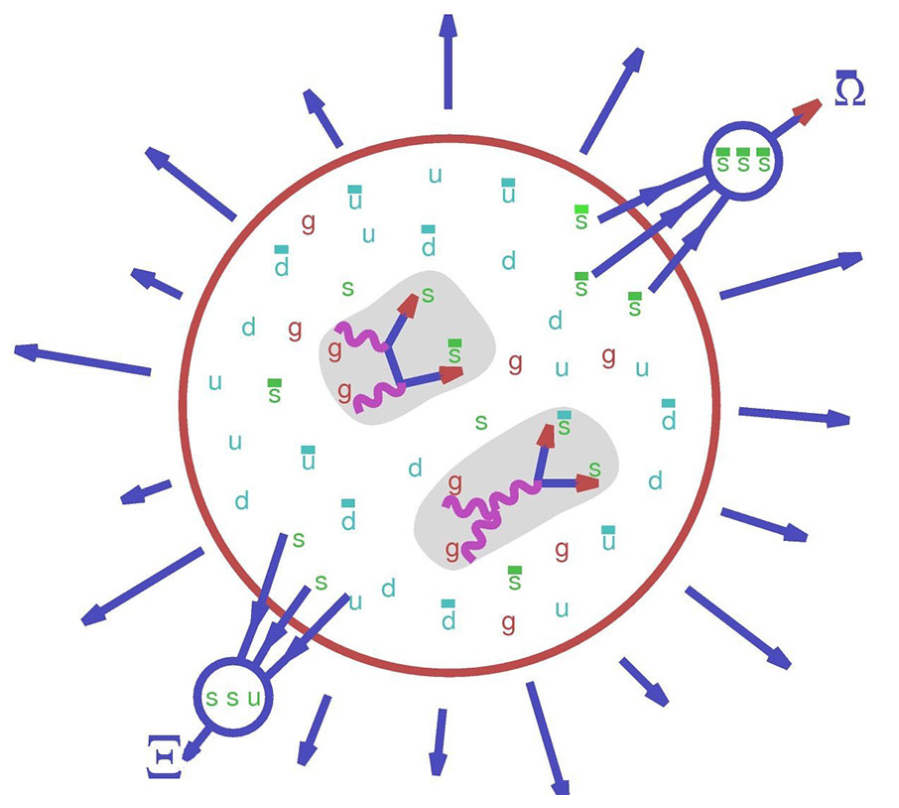
\includegraphics[width=0.7\textwidth]{strangeness-production.png}};
      \node[font=\tiny] at (1.8,-1.7) {\href{https://link.springer.com/article/10.1140/epja/i2015-15114-0}{Eur. Phys. J. A (2015) 51: 114}};
    \end{tikzpicture}

    \

    \begin{tikzpicture}
      \node{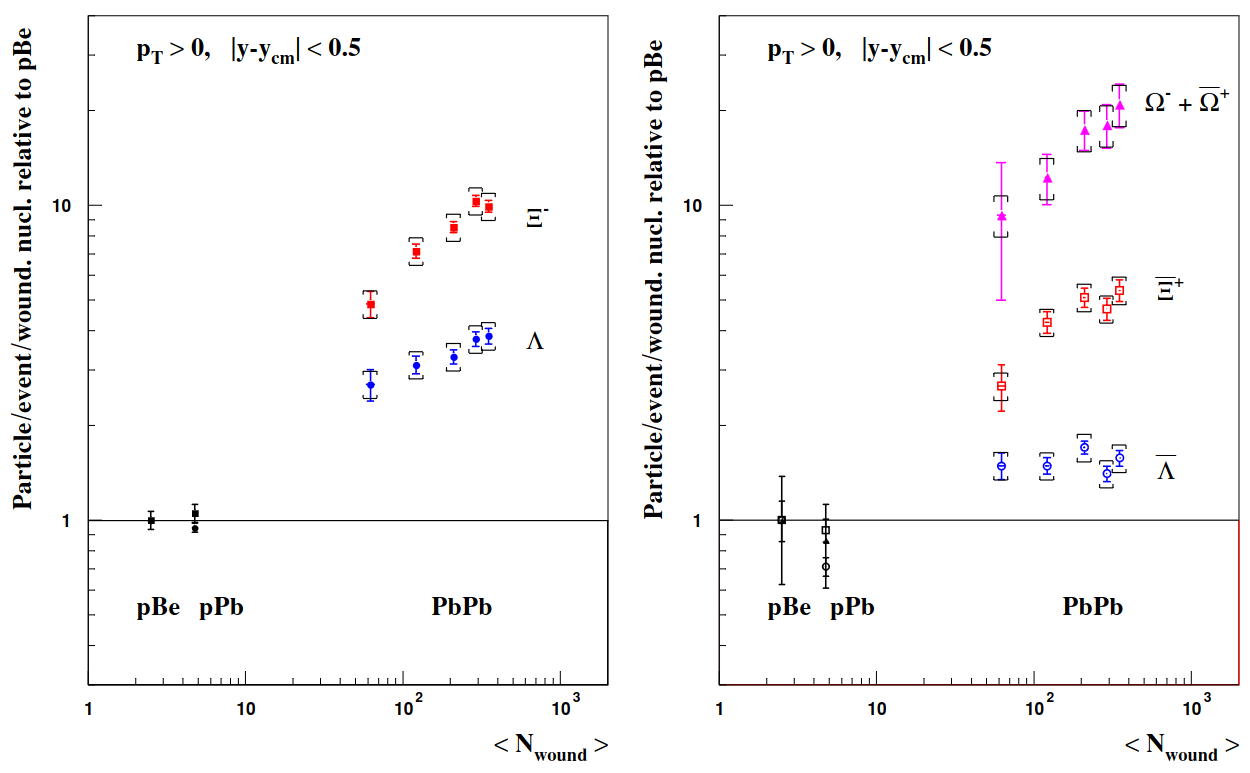
\includegraphics[width=1.0\textwidth]{strangeness-enhancement.png}};
      \node[font=\tiny] at (-0.5,2) {\textbf{Strangeness enhancement observed by NA57 at SPS (CERN)}};
      \node[font=\tiny] at (-1.6,-1.85) {\href{https://arxiv.org/abs/nucl-ex/0403016v2}{arXiv:nucl-ex/0403016}};
    \end{tikzpicture}

  \end{columns}


\end{frame}
